\documentclass{jsarticle}
\usepackage[dvipdfmx]{graphicx}
\usepackage{subcaption}
\captionsetup[figure]{justification=centering}
\captionsetup[table]{justification=centering}
\usepackage[ipa]{pxchfon}

\begin{document}
\title{{\vspace*{-30mm}}{\LARGE アドバンスドコントロール課題(レポート)}}
\author{\large 千葉工業大学 先進工学部 未来ロボティクス学科 \vspace*{4mm}\\20C1015 今井悠月}
\date{}
\maketitle\vspace*{10mm}

\section*{問1}
A = [0 1; -5 -6], \hspace*{0.5zw}B = [0; 1] のシステムに対して, 最適レギュレータを設計してください.\\
\hspace*{1zw}なお, Q = [1 0; 0 1], \hspace*{0.5zw}R = 1 とします.\\
\hspace*{1zw}以下のコマンドを入力してヘルプを見ながら最適レギュレータの状態フィードバック係数ベクトルを求めて
\hspace*{1zw}ください.\vspace*{2mm}\\
\hspace*{1zw}help lqr\\

\vspace*{4mm}\subsection*{解答}
help lqr を参照の元, コードを作成し, 実行した結果は以下の図1のようになった.\\
\hspace*{1zw}講義内での手計算によって求めた結果と同様になったため, 正しく最適レギュレータを設計できたといえる.\\

\begin{figure}[htbp]
  \begin{minipage}[t]{0.5\linewidth}
    \centering
    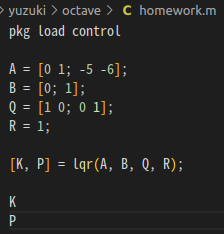
\includegraphics[keepaspectratio, scale=0.65]{fig/2.png}
    \subcaption{作成したコード}
  \end{minipage}
  \begin{minipage}[t]{0.5\linewidth}
    \centering
    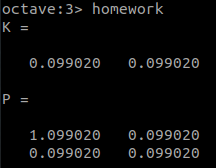
\includegraphics[keepaspectratio, scale=0.90]{fig/1.png}
    \subcaption{コード実行結果}
  \end{minipage}\vspace*{2mm}
  \caption{最適レギュレータの設計及び状態フィードバック係数ベクトルを求めるコード}
\end{figure}



\vspace*{1mm}\section*{問2}
初期値 x0 = [1; 0] として, 時間応答のグラフも求めてください.\\

\vspace*{4mm}\subsection*{解答}
上記で求めた, 最適レギュレータの状態フィードバック係数ベクトルを適用した時間応答のグラフは以下の\\
\hspace*{1zw}図2のようになった.\\

\begin{figure}[htbp]
  \begin{minipage}[t]{0.5\linewidth}
    \centering
    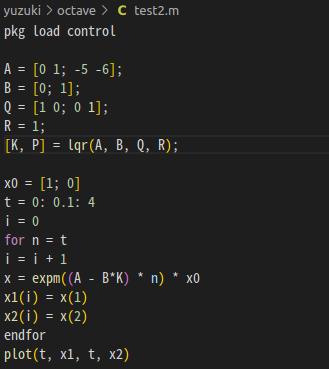
\includegraphics[keepaspectratio, scale=0.485]{fig/ato_c.png}
    \subcaption{作成したコード}
  \end{minipage}
  \begin{minipage}[t]{0.5\linewidth}
    \centering
    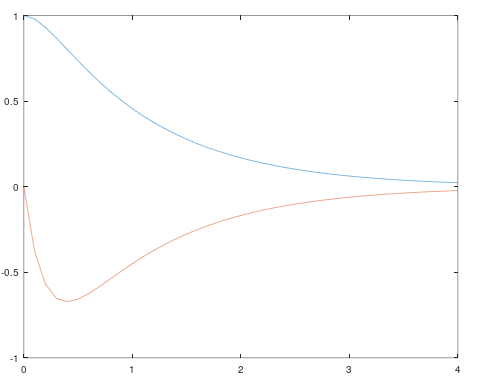
\includegraphics[keepaspectratio, scale=0.48]{fig/ato_r.png}
    \subcaption{時間応答のグラフ(コード実行結果)}
  \end{minipage}\vspace*{2mm}
  \caption{状態フィードバック係数ベクトル適用後の時間応答}
\end{figure}



\vspace*{2mm}
ここで, 最適レギュレータの設計により求めた, 状態フィードバック係数ベクトルを
適用する前(演習4)の\hspace*{1zw}時間応答のグラフを以下の図3に示す.\\

\begin{figure}[htbp]
  \begin{minipage}[t]{0.5\linewidth}
    \centering
    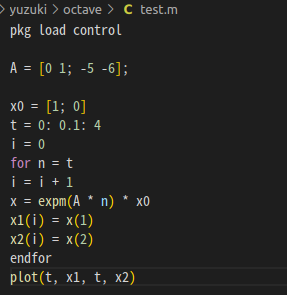
\includegraphics[keepaspectratio, scale=0.605]{fig/moto_c.png}
    \subcaption{講義内の演習4で作成したコード}
  \end{minipage}
  \begin{minipage}[t]{0.5\linewidth}
    \centering
    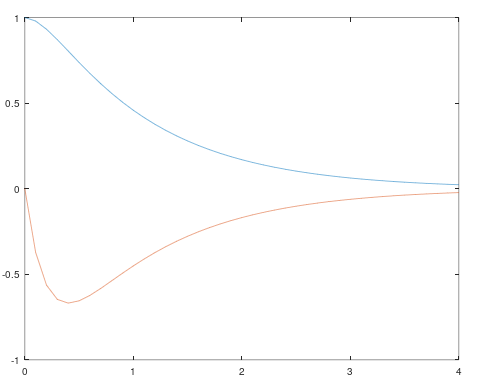
\includegraphics[keepaspectratio, scale=0.48]{fig/moto_r.png}
    \subcaption{時間応答のグラフ(コード実行結果)}
  \end{minipage}\vspace*{2mm}
  \caption{状態フィードバック係数ベクトル適用前の時間応答}
\end{figure}



図2と図3の時間応答のグラフを比較すると, 最適レギュレータの設計によって求めた状態フィードバック
\hspace*{1zw}係数ベクトルの適用後と適用前でグラフの概形が同じである.\\

このことから, 単純に状態フィードバック係数ベクトルを適用するだけでは, 望むような応答を得ることは\hspace*{1zw}できず, 
システムによって適切なQ と R の値を設定することが必要であるとわかる.

\section*{問3}
また, Q, R をどのような値にするとより早く収束するか.\\
\hspace*{1zw}いくつか Q, R の組に対する応答を示しながら解説せよ.\\

\vspace*{4mm}\subsection*{解答}
まずは, R の値を1に固定し, Q の (1, 1)成分の値を可変にして, どのような傾向があるかを調査する.

\begin{figure}[h!]
  \centering
  \begin{minipage}{0.325\linewidth}
    \centering
    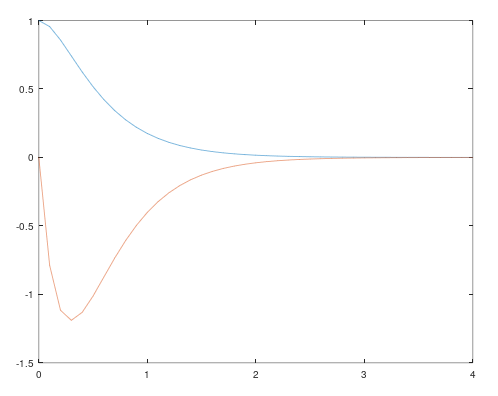
\includegraphics[width=\linewidth]{./fig/q100_r1.png}
    \caption{Q = 100, R = 1}
  \end{minipage}
  \hfill
  \begin{minipage}{0.325\linewidth}
    \centering
    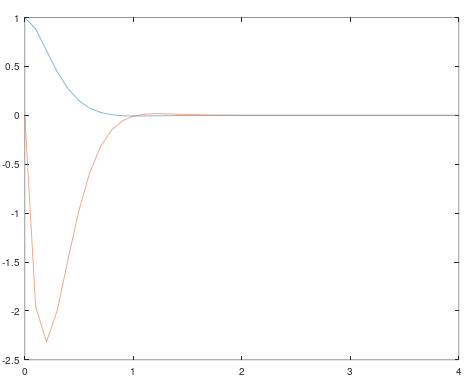
\includegraphics[width=\linewidth]{./fig/q1000_r1.png}
    \caption{Q = 1000, R = 1}
  \end{minipage}
  \hfill
  \begin{minipage}{0.325\linewidth}
    \centering
    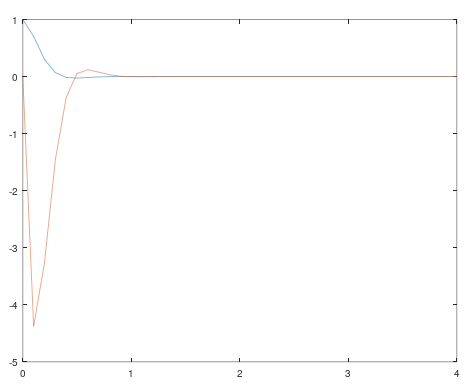
\includegraphics[width=\linewidth]{./fig/q10000_r1.png}
    \caption{Q = 10000, R = 1}
  \end{minipage}
\end{figure}

これらの結果から Q の値(第一成分)を大きくすると収束が早まることがわかる.\\
\hspace*{1zw}しかし, 図5 と 図6の結果の比較より, 値が大きすぎても逆に収束が遅くなってしまうことがわかる.\\
\hspace*{1zw}すなわち, どこかの値で収束する限界が存在し, それ以降の値は逆効果になると考えられる.\\

次に Q の値を固定し, Rの値を可変にして, 同様に傾向を調査する.

\begin{figure}[h!]
  \centering
  \begin{minipage}{0.325\linewidth}
    \centering
    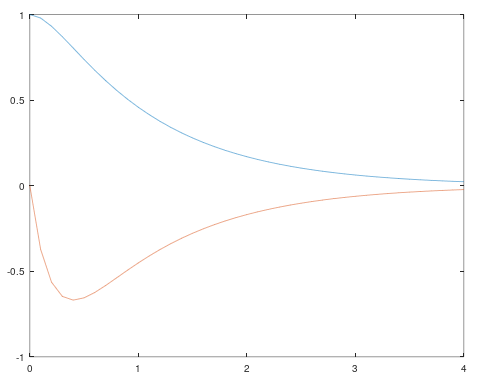
\includegraphics[width=\linewidth]{./fig/q1_r100.png}
    \caption{Q = 1, R = 100}
  \end{minipage}
  \hfill
  \begin{minipage}{0.325\linewidth}
    \centering
    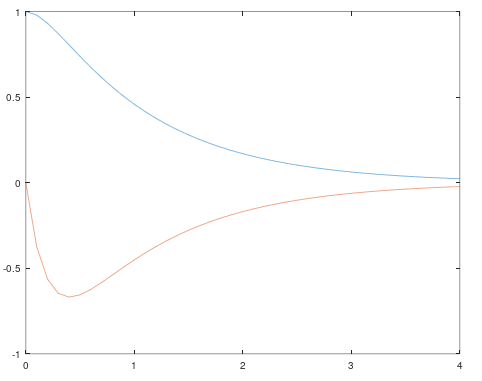
\includegraphics[width=\linewidth]{./fig/q1_r1000.png}
    \caption{Q = 1, R = 1000}
  \end{minipage}
  \hfill
  \begin{minipage}{0.325\linewidth}
    \centering
    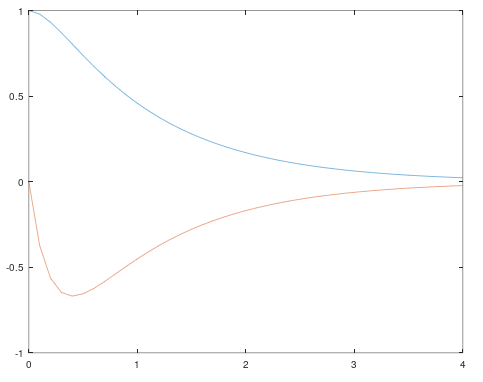
\includegraphics[width=\linewidth]{./fig/q1_r10000.png}
    \caption{Q = 1, R = 10000}
  \end{minipage}
\end{figure}

これらの結果から Q の値を固定し, R の値のみを可変にしても変化は起こらないことがわかる.\\
\hspace*{1zw}このことから, R の値は, Q の値と組み合わせて両者を可変にすることで効力を発揮すると予想できる.\\

\vspace*{10mm}
よって, 今度は Q と R の値の両者を可変にして, どのような値にすると収束が早まるかを調査する.






\end{document}
